In this section the experimental validation is carried out, showing that controlling the diversity in the variable space is a way to improve further some of the results obtained by state-of-art-MOEAs.% which belong to jMetalcpp~\cite{Joel:JMETAL} framework.
%
In the same way, the scalability of each algorithm is analyzed with respect an increasing number of decision variables.
%
The WFG \cite{Joel:WFG}, DTLZ \cite{Joel:DTLZ}  and UF \cite{Joel:CEC2009}  test problems have been used for our purpose. 
%

Through the literature several crossover operators have been proposed in MOEAs~\cite{Joel:ParentMeanCentricSelfAdaptation},  
a popular operator is the Simulated Binary Crossover (SBX).4\cite{Joel:SBX1994}%, Joel:TAXONOMY_CROSSOVER, Joel:Kalyanmoy}
%	
In addition based in diversity-related properties the No-Reflection Dynamic SBX is implemented \cite{Joel:DNR_SBX}, which is considered as a variant of the SBX operator.


%
Additionally, our experimental validation includes the VSD-MOEA, as well as four well-known state-of-the-art algorithms.
%
Given that all of them are stochastic algorithms, each execution was repeated 35 times with different seeds.
%
The common configuration in all of them was the following: the stopping criterion was set to $250,000$ generations, the population size was fixed to 100, the WFG test problems were configured with two and three objectives, setting 24 parameters, where 20 of them are distance parameters and 4 are position parameters.
%
Specifically, in the DTLZ test instances, the number of decision variables is set to $n=M+r-1$, where $r=\{5, 10, 20\}$ for DTLZ1, DTLZ2 to DTLZ6 and DTLZ7 respectively, as is suggested by the authors \cite{Joel:DTLZ}.  
% 
The UF benchmark is composed of ten test instances, where the first seven are of two objectives and the rest with three objectives, the number of decision variables is assigned to $n=10$.

%
In general (except for GDE3), the crossover and mutation operators are DNR-SBX and polynomial respectively, with crossover probability of 0.9 and mutation of $1/n$  \cite{Joel:Mutation}, also the crossover and mutation distribution indexes were assigned to 20 and 50 respectively.
%
The extra-parametrization of each algorithm is showed in the table \ref{tab:Parametrization}.
%

\begin{table}[t]
\centering
\caption{Parametrization}
\label{tab:Parametrization}
\begin{tabular}{l|l}
\hline
\textbf{Algorithm} & \textbf{Configuration} \\ \hline
GDE3 & CR = 0.9 and F = 0.5 \\ \hline
MOMBI-II & $\epsilon = 1e-3$, $\alpha = 0.5$, record size = 5 generations \\ \hline
MOEA/D & \begin{tabular}[c]{@{}l@{}}size of neighborhood,= 20, \\ max updates by sub-problem (nr) = 2 and $\delta = 0.9$\end{tabular} \\ \hline
VSD-MOEA & $D_I=\sqrt{n}*0.25$ \\ \hline
\end{tabular}
\end{table}

%\begin{itemize}
% %\scriptsize
% \item \textbf{GDE3}: CR = 0.9 and F = 0.5.
% \item \textbf{MOMBI-II}: $\epsilon = 1e-3$, $\alpha = 0.5$, record size = 5 generations. 
% \item \textbf{MOEA/D}: size of neighborhood  = 20, max updates by sub-problem (nr) = 2 and $\delta = 0.9$.
% \item \textbf{VSD-MOEA}: $D_I=\sqrt{n}*0.25$.
% \end{itemize}

Particularly, the algorithms MOEA/D and MOMBI-II require a set of vectors uniformly scattered on the unit-simplex, therefore the number of vectors generated increases nonlinearly with the number of objectives.
%
Consequently, is applied the method proposed in \cite{Joel:MOEAD_Uniform_Design, Joel:Kuhn_Munkres} where the uniform design (UD) \cite{Joel:Uniform_Design} and good lattice point (glp) are combined.
%
Thus the number weight of vectors is not affected by the number of objectives.

In addition, our experimental analysis has been carry out with the hypervolume indicator, since the WFG benchmark variate the Pareto front shape with different distance parameters \cite{Joel:ScalabilityStudy}.
%

In this work the reference points are chosen to be a vector with values slightly larger than the nadir point, also for complex problems the reference point is considered as nadir point plus the unity.
%
Therefore the reference points implemented in the hypervolume indicator are showed in the table \ref{tab:ReferencePoints} as used in \cite{Joel:Kuhn_Munkres, Joel:OperatorAHX}.

\begin{table}[t]
\centering
\caption{References points for the HV indicator}
\label{tab:ReferencePoints}
\begin{tabular}{cc}
\hline
\textbf{Instances} & \textbf{Reference Point} \\ \hline
WFG1-WFG9 & $[2.1, ...,2m+0.1]$ \\
DTLZ 1, 2, 4 & $[1.1, ..., 1.1]$ \\
DTLZ 3, 5, 6 & $[3, ..., 3]$ \\
DTLZ7 & $[1.1, ..., 1.1, 2m]$ \\
UF 1-10 & $[2, ..., 2]$ \\ \hline
\end{tabular}
\end{table}
%
In order to statistically compare the hypervolume results, a similar guideline than the proposed in~\cite{Joel:StatisticalTest} was used. 
%
First a Shapiro-Wilk test was performed to check whatever or not the values of the results followed a Gaussian distribution. 
%
If, so, the Levene test was used to check for the homogeneity of the variances. 
%
If samples had equal variance, an ANOVA test was done; if not, a Welch test was performed. 
%
For non-Gaussian distributions, the nonparametric Kruskal-Wallis test was used to test whether samples are drawn from the same distribution. 
%
An algorithm $X$ is said to win algorithm $Y$ when the differences between them are statistically significant, if the mean and median obtained by $X$ are higher than the mean and median achieved by $Y$.

%

In the tables \ref{tab:StatisticsHV_2obj}, \ref{tab:StatisticsHV_3obj} are showed the hypervolume statistics with two an three objectives respectively.
%
The column \textit{Diff} indicate how far is the best HV mean from each algorithm, this field is computed as the difference between the mean of the each algorithm and the best mean.
%
Consequently, the best algorithm in each instance has assigned a zero.
%

Considering two objectives the GDE3 provides the best results, however the VSD-MOEA is very close to the GDE3 as is showed in the \textit{Diff} columns.
%
It is important to highlight that the DTLZ test suites have the next weaknesses \cite{Joel:CEC2009}.
The global optimum lies in the center or bounds, all are separable and the global optimum has the same parameter values for different dimensions.
%
Particularly the DTLZ5 and DTLZ6 are easy for the GDE3, since the global optimal are located in the low bound, thus if the differential operators locate a solution outside of bounds, the repair procedure could move the point among the optimal.

%
Additionally, the GDE3 get worse according increases the number of objectives, even more the \textit{Diff} results are in average high, except for the DTLZ5 and DTLZ6 where the optimal set are located along the bounds.
%
Despite the fact that the VSD-MOEA does not have a repair procedure because it implements genetic operators, the results are fairly stable.
%
Also improves the hypervolume with three objectives, hence can be considered a robust algorithm, in fact considering more objectives it provides better results than the dominance-based algorithms\footnote{Experimentally with ten objectives the algorithm is best than dominance-based MOEAs.}.
%
A remarkable characteristic that can be appreciated in two and three objectives is that our  proposal provide the best results in the most difficult problems as are dependence, multi-modal and deceptiveness.

%
On average the VSD-EMOA has lower \textit{Diff} value than the rest of algorithms, therefore considering all best mean of each instance, the VSD-EMOA is not too far from the best means.
%
Even more, the min and max averages are better than the min and max of the state-of-art algorithms.
%

The effective test showed in the tables \ref{tab:Effective_Test_2obj}, \ref{tab:Effective_Test_3obj} are conformed by two an three objectives respectively,  these metrics qualify the superiority of each algorithm with the rest through pair comparisons.
%
Thus, an algorithm \textbf{A} is compared with algorithm \textbf{B}, if \textbf{A} wins, the difference with \textbf{B} is accumulated in wins $\uparrow$ of the algorithm \textbf{A}, the same process is for the algorithm \textbf{B} but it is accumulated in the lost field $\downarrow$.
%
The column \textit{Score} is conformed by the difference between the win and lost values, therefore a high positive score indicate the superiority of the algorithm.
%

In addition, our proposal has low negative scores in the DTLZ6 and WFG6 with two objectives, it might occurs because these instances are not a problem to long term executions, therefore they are totally defined by the crowding procedure.
%
However, the negative scores in VSD-MOEA are not highly significant.
%
Additionally, considering three objectives, the VSD-MOEA provides the best and positive scores.
%
In general our proposal has the best scores in difficult instances as are the UF and some WFG problems.



\subsection{Decision Variable Scalability Experiments}

The scalability of each MOEA is also evaluated respect with the number of decision variables \cite{Joel:ScalabilityStudy}. 
%
The figures \ref{fig:Scalability_Study_HV_1}, \ref{fig:Scalability_Study_HV_2} show the hypervolume performance of 30, 100, 250 and 500 variables respectively.
%
Particularly,  the scalability study was realized in DTLZ4, UF5 with two objectives and DTLZ4, UF10 with three objectives.
%
In some instances the GDE3 degrades relatively fast according increases the number of decision variables as is showed in UF5, UF10 and DTLZ4 with three objectives.
%
Also, the GDE3 show a non-stable performance with the parameter configurations, as is explained by J. Lampinen et al.\cite{Joel:GDE3_CEC09}, where they indicate that a high value for CR might lead to premature convergence with respect to one objective compared to another.

%
Specifically, the instance UF10 with GDE3 has an increment of HV for 100 variables, this irregularity is related with diversity issues \cite{Joel:GDE3_CEC09}
%
On the other hand the VSD-MOEA is enough stable, also it provides the best HV values.
%
It is interesting that the MOEA/D and MOMBI-II required an extra-parametrization, hence the stability could be compromised.

%
The 50\% attainment surfaces WFG2, WFG8 and DTLZ7 instances are showed in the figure \ref{fig:Attainment_Surfaces}.
%
The analyses shows that our proposal provide solutions approximated to the Pareto front.
%
Although the GDE3 approximate the WFG2 and DTLZ7, this this algorithm is far in some regions of the Pareto front with the WFG8 instance. 

\begin{figure*}[t]
\centering
\caption{Scalability study of decision variables with two objectives (HV)}
\label{fig:Scalability_Study_HV_1}
\begin{tabular}{cc}
   \includegraphics[width=0.25\textwidth, angle=-90,origin=c]{Images/DTLZ4_2obj.eps} &
    \includegraphics[width=0.25\textwidth, angle=-90,origin=c]{Images/UF5.eps}  
\end{tabular}
\end{figure*}
\begin{figure*}[t]
\centering
\caption{Scalability study of decision variables with three objectives (HV)}
\label{fig:Scalability_Study_HV_2}
\begin{tabular}{cc}
    \includegraphics[width=0.25\textwidth, angle=-90,origin=c]{Images/DTLZ4_3obj.eps} &
    \includegraphics[width=0.25\textwidth, angle=-90,origin=c]{Images/UF10.eps}
\end{tabular}
\end{figure*}
\begin{figure*}[t]
\centering
\caption{50\% Attainment Surfaces Achieved}
\label{fig:Attainment_Surfaces}
\begin{tabular}{ccc}
   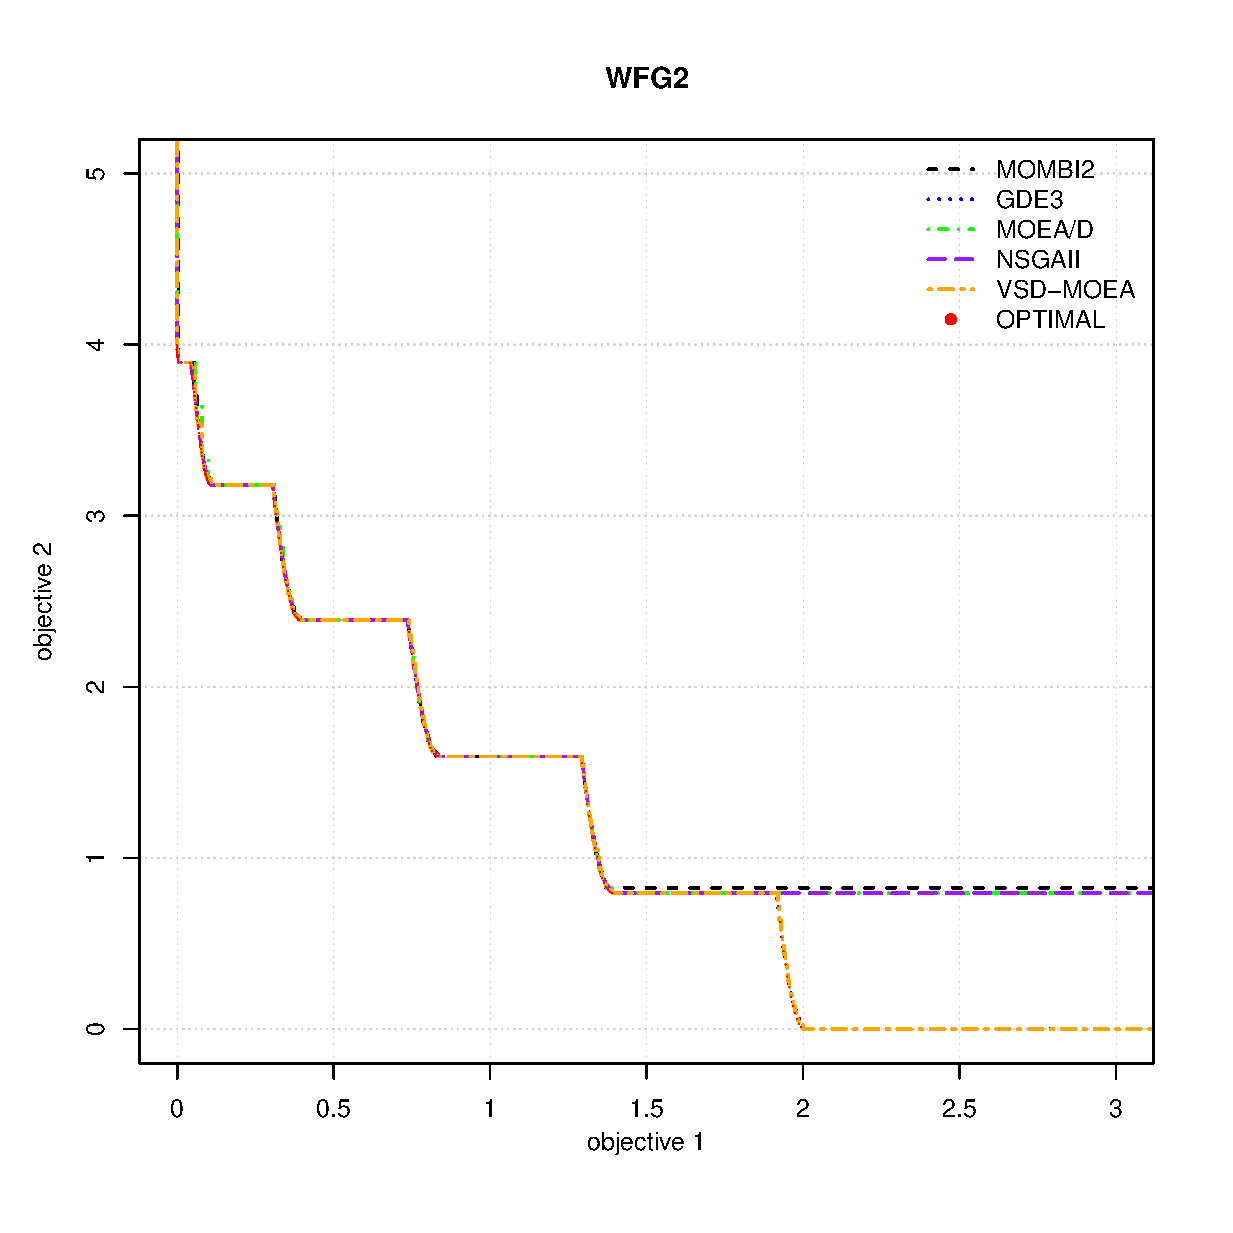
\includegraphics[width=0.33\textwidth]{Surfaces/WFG2.eps} &
    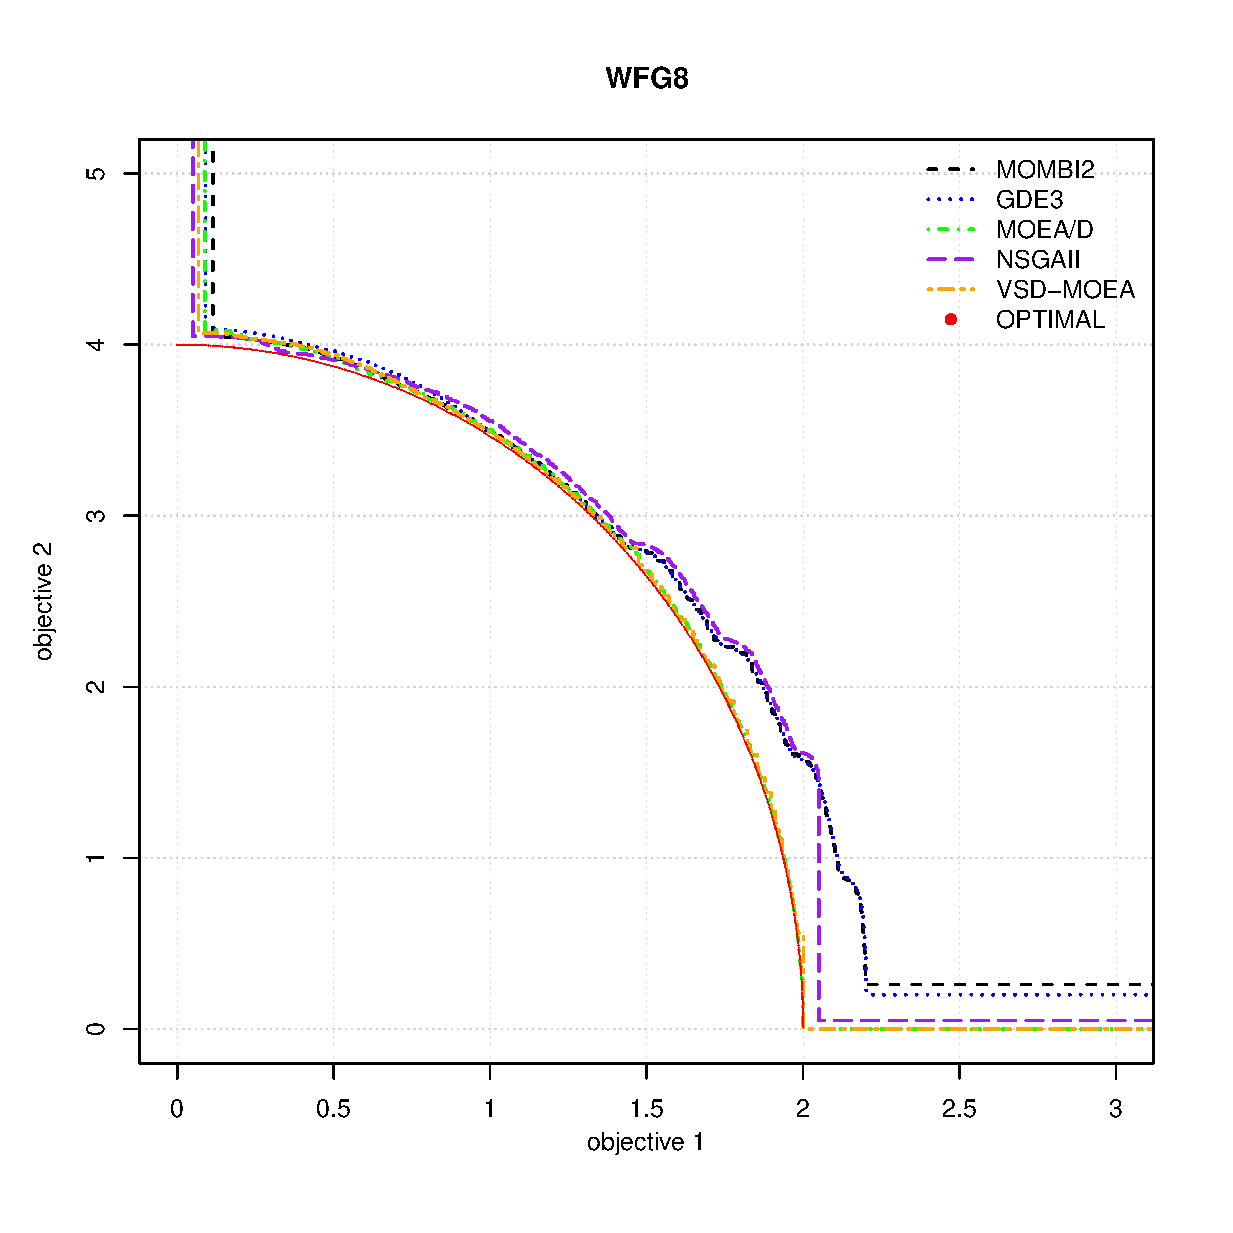
\includegraphics[width=0.33\textwidth]{Surfaces/WFG8.eps} &
     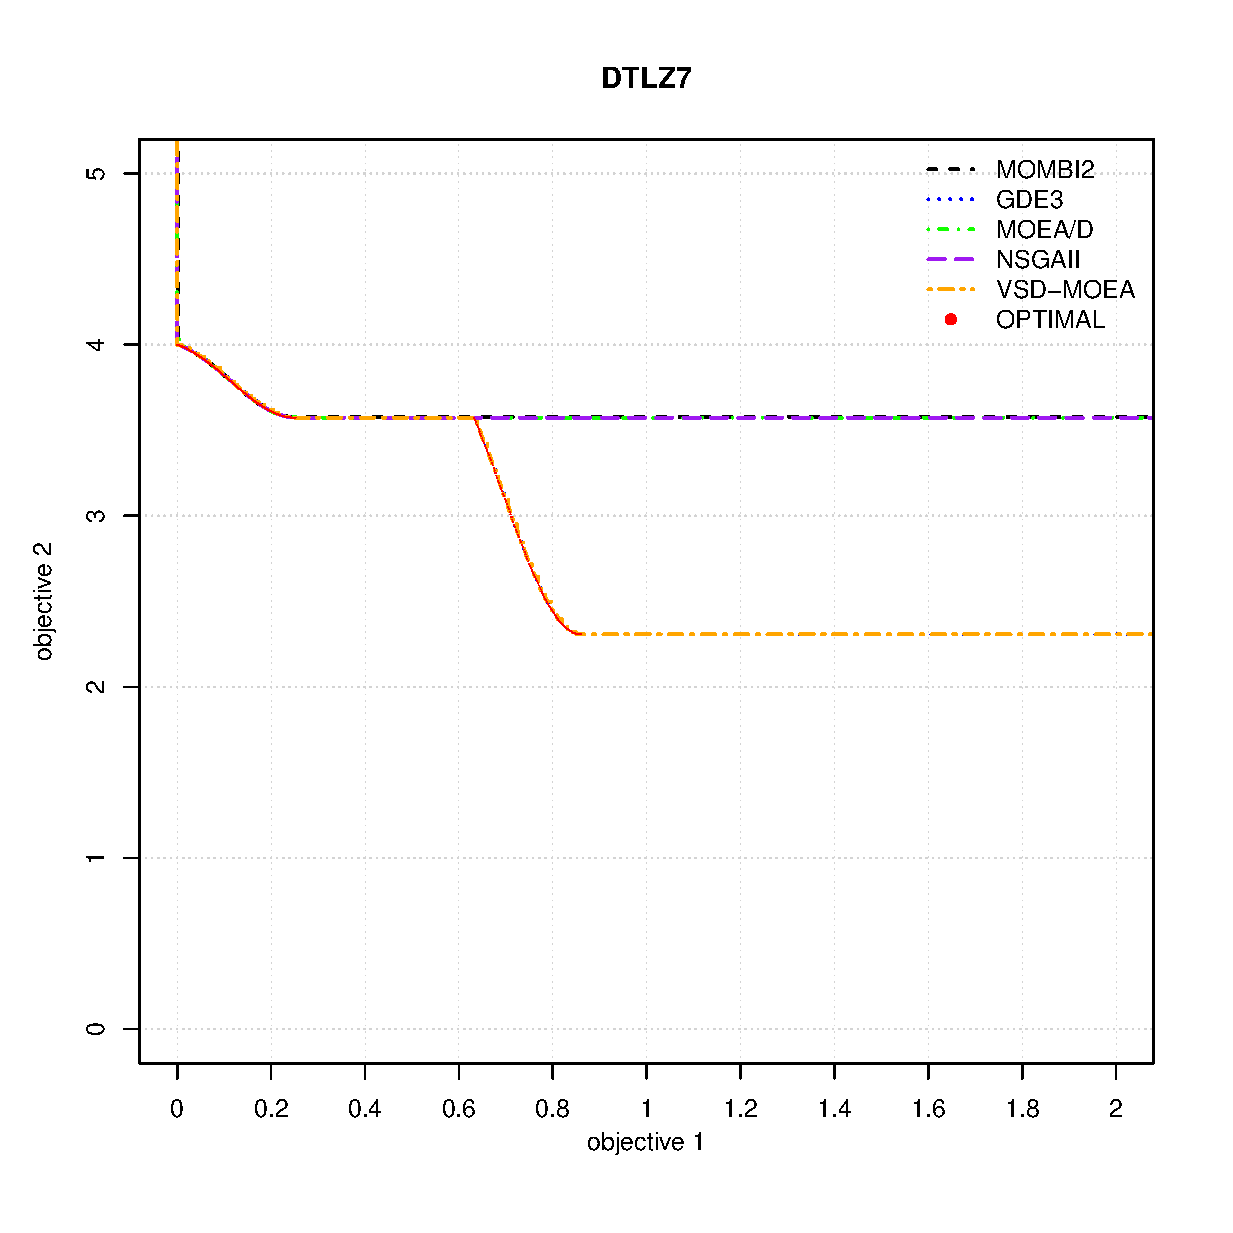
\includegraphics[width=0.33\textwidth]{Surfaces/DTLZ7.eps}
\end{tabular}
\end{figure*}
%%%%%%%%%%%%%%%%%%%%%
%
% Please add the following required packages to your document preamble:
% \usepackage{graphicx}
\begin{table*}[t]
\centering
\caption{Statistics HV with two objectives}
\label{tab:StatisticsHV_2obj}
\resizebox{\textwidth}{!}{%
 \begin{threeparttable}
\begin{tabular}{c|c|c|c|c|c|c|c|c|c|c|c|c|c|c|c|c|c|c|c|c}
\cline{2-21}
                              & \multicolumn{4}{c|}{GDE3}                       & \multicolumn{4}{c|}{MOMBI-II}                   & \multicolumn{4}{c|}{NSGAII}            & \multicolumn{4}{c|}{MOEA/D}            & \multicolumn{4}{c}{VSD-MOEA}                   \\ \cline{2-21} 
                              & Min   & Max   & Mean           & Diff           & Min   & Max   & Mean           & Diff           & Min   & Max   & Mean  & Diff           & Min   & Max   & Mean  & Diff           & Min   & Max   & Mean           & Diff           \\ \hline
\multicolumn{1}{c|}{DTLZ1}   & 1.084 & 1.084 & \textbf{1.084} & 0.000          & 1.078 & 1.078 & 1.078          & 0.006          & 1.083 & 1.083 & 1.083 & 0.000          & 1.078 & 1.084 & 1.081 & 0.003          & 1.084 & 1.084 & \textbf{1.084} & 0.000          \\ \hline
\multicolumn{1}{c|}{DTLZ2}   & 0.421 & 0.421 & \textbf{0.421} & 0.000          & 0.418 & 0.418 & 0.418          & 0.003          & 0.419 & 0.420 & 0.419 & 0.001          & 0.420 & 0.420 & 0.420 & 0.001          & 0.420 & 0.420 & 0.420          & 0.000          \\ \hline
\multicolumn{1}{c|}{DTLZ3}   & 8.211 & 8.211 & \textbf{8.211} & 0.000          & 8.170 & 8.170 & 8.170          & 0.041          & 8.209 & 8.210 & 8.209 & 0.001          & 8.169 & 8.210 & 8.200 & 0.011          & 8.210 & 8.210 & 8.210          & 0.000          \\ \hline
\multicolumn{1}{c|}{DTLZ4}   & 0.421 & 0.421 & \textbf{0.421} & 0.000          & 0.110 & 0.418 & 0.383          & 0.038          & 0.110 & 0.420 & 0.313 & 0.107          & 0.110 & 0.418 & 0.365 & 0.055          & 0.420 & 0.420 & 0.420          & 0.000          \\ \hline
\multicolumn{1}{c|}{DTLZ5}   & 8.211 & 8.211 & \textbf{8.211} & 0.000          & 8.170 & 8.170 & 8.170          & 0.041          & 8.209 & 8.210 & 8.209 & 0.001          & 8.210 & 8.210 & 8.210 & 0.001          & 8.210 & 8.210 & \textbf{8.210} & 0.000          \\ \hline
\multicolumn{1}{c|}{DTLZ6}   & 8.211 & 8.211 & \textbf{8.211} & 0.000          & 7.989 & 8.170 & 8.073          & 0.138          & 8.062 & 8.209 & 8.128 & 0.083          & 8.027 & 8.210 & 8.095 & 0.116          & 7.989 & 8.210 & 8.123          & 0.088          \\ \hline
\multicolumn{1}{c|}{DTLZ7}   & 0.894 & 0.894 & \textbf{0.894} & 0.000          & 0.417 & 0.417 & 0.417          & 0.478          & 0.420 & 0.420 & 0.420 & 0.474          & 0.420 & 0.420 & 0.420 & 0.474          & 0.893 & 0.893 & 0.893          & 0.001          \\ \hline
\multicolumn{1}{c|}{UF1}     & 3.657 & 3.659 & 3.658          & 0.002          & 3.327 & 3.517 & 3.490          & 0.171          & 3.650 & 3.652 & 3.651 & 0.010          & 3.428 & 3.660 & 3.588 & 0.072          & 3.655 & 3.662 & \textbf{3.661} & 0.000          \\ \hline
\multicolumn{1}{c|}{UF2}     & 3.651 & 3.654 & 3.653          & 0.005          & 3.406 & 3.628 & 3.594          & 0.064          & 3.643 & 3.647 & 3.645 & 0.013          & 3.428 & 3.649 & 3.533 & 0.124          & 3.655 & 3.660 & \textbf{3.658} & 0.000          \\ \hline
\multicolumn{1}{c|}{UF3}     & 3.371 & 3.660 & \textbf{3.642} & 0.000          & 3.328 & 3.595 & 3.499          & 0.143          & 3.524 & 3.639 & 3.602 & 0.041          & 2.850 & 3.642 & 3.451 & 0.191          & 3.549 & 3.620 & 3.593          & 0.049          \\ \hline
\multicolumn{1}{c|}{UF4}     & 3.219 & 3.237 & 3.224          & 0.036          & 3.194 & 3.205 & 3.197          & 0.062          & 3.198 & 3.207 & 3.200 & 0.060          & 3.210 & 3.243 & 3.228 & 0.032          & 3.235 & 3.280 & \textbf{3.260} & 0.000          \\ \hline
\multicolumn{1}{c|}{UF5}     & 2.532 & 3.000 & \textbf{2.964} & 0.000          & 2.047 & 2.746 & 2.522          & 0.442          & 1.861 & 2.897 & 2.602 & 0.362          & 1.800 & 2.550 & 2.185 & 0.778          & 2.591 & 3.267 & 2.951          & 0.013          \\ \hline
\multicolumn{1}{c|}{UF6}     & 2.000 & 3.325 & \textbf{3.098} & 0.000          & 2.013 & 2.893 & 2.638          & 0.460          & 2.007 & 2.896 & 2.518 & 0.580          & 0.726 & 2.884 & 2.070 & 1.028          & 2.893 & 3.306 & 3.058          & 0.040          \\ \hline
\multicolumn{1}{c|}{UF7}     & 3.490 & 3.492 & \textbf{3.491} & 0.000          & 2.474 & 3.470 & 2.592          & 0.899          & 2.168 & 3.485 & 3.190 & 0.301          & 2.015 & 3.493 & 2.743 & 0.748          & 3.473 & 3.493 & 3.489          & 0.002          \\ \hline
\multicolumn{1}{c|}{WFG1}    & 4.263 & 5.256 & 4.848          & 0.408          & 4.623 & 5.666 & \textbf{5.256} & 0.000          & 4.716 & 5.250 & 5.156 & 0.100          & 4.480 & 5.243 & 5.037 & 0.219          & 4.717 & 5.250 & 5.205          & 0.051          \\ \hline
\multicolumn{1}{c|}{WFG2}    & 5.072 & 5.072 & \textbf{5.072} & 0.000          & 4.925 & 4.942 & 4.927          & 0.145          & 4.948 & 5.068 & 4.953 & 0.119          & 4.943 & 4.943 & 4.943 & 0.128          & 5.069 & 5.069 & 5.069          & 0.003          \\ \hline
\multicolumn{1}{c|}{WFG3}    & 4.513 & 4.530 & 4.522          & 0.043          & 4.561 & 4.563 & 4.562          & 0.003          & 4.533 & 4.543 & 4.539 & 0.026          & 4.562 & 4.563 & 4.563 & 0.002          & 4.565 & 4.565 & \textbf{4.565} & 0.000          \\ \hline
\multicolumn{1}{c|}{WFG4}    & 2.280 & 2.286 & 2.283          & 0.009          & 2.284 & 2.285 & 2.285          & 0.007          & 2.271 & 2.283 & 2.277 & 0.014          & 2.287 & 2.287 & 2.287 & 0.005          & 2.291 & 2.291 & \textbf{2.291} & 0.000          \\ \hline
\multicolumn{1}{c|}{WFG5}    & 1.984 & 1.990 & \textbf{1.986} & 0.000          & 1.976 & 1.996 & 1.980          & 0.005          & 1.970 & 1.977 & 1.975 & 0.011          & 1.972 & 2.010 & 1.977 & 0.009          & 1.976 & 1.984 & 1.980          & 0.005          \\ \hline
\multicolumn{1}{c|}{WFG6}    & 2.092 & 2.246 & \textbf{2.183} & 0.000          & 2.055 & 2.207 & 2.141          & 0.043          & 2.059 & 2.207 & 2.138 & 0.046          & 2.017 & 2.188 & 2.129 & 0.054          & 2.082 & 2.198 & 2.131          & 0.053          \\ \hline
\multicolumn{1}{c|}{WFG7}    & 2.272 & 2.280 & 2.276          & 0.015          & 2.284 & 2.285 & 2.284          & 0.007          & 2.269 & 2.282 & 2.275 & 0.016          & 2.287 & 2.287 & 2.287 & 0.005          & 2.291 & 2.291 & \textbf{2.291} & 0.000          \\ \hline
\multicolumn{1}{c|}{WFG8}    & 1.860 & 1.876 & 1.868          & 0.363          & 1.868 & 2.237 & 1.951          & 0.280          & 1.803 & 2.140 & 1.906 & 0.325          & 1.938 & 2.252 & 2.225 & 0.006          & 2.050 & 2.248 & \textbf{2.231} & 0.000          \\ \hline
\multicolumn{1}{c|}{WFG9}    & 1.711 & 1.714 & 1.713          & 0.542          & 2.197 & 2.264 & 2.244          & 0.010          & 2.168 & 2.258 & 2.229 & 0.026          & 1.706 & 2.264 & 2.225 & 0.030          & 2.242 & 2.271 & \textbf{2.255} & 0.000          \\ \hline
\multicolumn{1}{c|}{Average} & 3.279 & 3.423 & 3.388          & \textbf{0.062} & 3.170 & 3.406 & 3.299          & \textbf{0.151} & 3.187 & 3.409 & 3.332 & \textbf{0.118} & 3.047 & 3.397 & 3.272 & \textbf{0.178} & 3.372 & 3.474 & 3.437          & \textbf{0.013} \\ \hline
\end{tabular}
 \begin{tablenotes}
      \small
      \item The bold values correspond to the best HV mean of each instance, in case of repeated they are also in bold.
    \end{tablenotes}
    \end{threeparttable}
}
\end{table*}



% Please add the following required packages to your document preamble:
% \usepackage{graphicx}
\begin{table*}[t]
\centering
\caption{Statistics HV with three objectives}
\label{tab:StatisticsHV_3obj}
\resizebox{\textwidth}{!}{%
 \begin{threeparttable}
\begin{tabular}{c|c|c|c|c|c|c|c|c|c|c|c|c|c|c|c|c|c|c|c|c}
\cline{2-21}
 & \multicolumn{4}{c|}{GDE3} & \multicolumn{4}{c|}{MOMBI-II} & \multicolumn{4}{c|}{NSGAII} & \multicolumn{4}{c|}{MOEA/D} & \multicolumn{4}{c}{VSD-MOEA} \\ \cline{2-21} 
 & Min & Max & Mean & Diff & Min & Max & Mean & Diff & Min & Max & Mean & Diff & Min & Max & Mean & Diff & Min & Max & Mean & Diff \\ \hline
\multicolumn{1}{c|}{DTLZ1} & 1.301 & 1.303 & 1.302 & 0.002 & 1.290 & 1.290 & 1.290 & 0.015 & 1.300 & 1.302 & 1.301 & 0.003 & 1.280 & 1.294 & 1.292 & 0.013 & 1.304 & 1.305 & \textbf{1.304} & 0.000 \\ \hline
\multicolumn{1}{c|}{DTLZ2} & 0.707 & 0.724 & 0.713 & 0.031 & 0.724 & 0.724 & 0.724 & 0.020 & 0.691 & 0.724 & 0.709 & 0.035 & 0.709 & 0.709 & 0.709 & 0.035 & 0.742 & 0.746 & \textbf{0.744} & 0.000 \\ \hline
\multicolumn{1}{c|}{DTLZ3} & 26.368 & 26.389 & 26.380 & 0.033 & 26.154 & 26.155 & 26.154 & 0.259 & 26.362 & 26.389 & 26.378 & 0.035 & 26.171 & 26.274 & 26.267 & 0.146 & 26.413 & 26.414 & \textbf{26.413} & 0.000 \\ \hline
\multicolumn{1}{c|}{DTLZ4} & 0.707 & 0.720 & 0.714 & 0.031 & 0.455 & 0.724 & 0.701 & 0.044 & 0.121 & 0.726 & 0.699 & 0.046 & 0.121 & 0.705 & 0.603 & 0.142 & 0.744 & 0.745 & \textbf{0.745} & 0.000 \\ \hline
\multicolumn{1}{c|}{DTLZ5} & 23.987 & 23.987 & \textbf{23.987} & 0.000 & 23.813 & 23.819 & 23.814 & 0.173 & 23.978 & 23.982 & 23.981 & 0.006 & 23.878 & 23.878 & 23.878 & 0.109 & 23.986 & 23.986 & 23.986 & 0.001 \\ \hline
\multicolumn{1}{c|}{DTLZ6} & 23.987 & 23.987 & \textbf{23.987} & 0.000 & 23.358 & 23.813 & 23.576 & 0.411 & 23.701 & 23.979 & 23.817 & 0.170 & 23.268 & 23.713 & 23.533 & 0.454 & 23.482 & 23.986 & 23.737 & 0.250 \\ \hline
\multicolumn{1}{c|}{DTLZ7} & 1.783 & 1.841 & 1.815 & 0.054 & 0.901 & 0.904 & 0.902 & 0.967 & 0.895 & 0.907 & 0.903 & 0.967 & 0.900 & 0.907 & 0.905 & 0.964 & 1.864 & 1.880 & \textbf{1.869} & 0.000 \\ \hline
\multicolumn{1}{c|}{UF10} & 0.010 & 3.886 & 0.658 & 6.232 & 3.148 & 5.585 & 3.961 & 2.929 & 3.762 & 6.260 & 4.660 & 2.230 & 2.914 & 4.079 & 3.554 & 3.336 & 6.000 & 7.237 & \textbf{6.890} & 0.000 \\ \hline
\multicolumn{1}{c|}{UF8} & 0.052 & 4.855 & 1.973 & 5.416 & 4.000 & 7.358 & 6.907 & 0.482 & 7.156 & 7.267 & 7.231 & 0.158 & 4.000 & 7.321 & 6.414 & 0.975 & 7.316 & 7.413 & \textbf{7.389} & 0.000 \\ \hline
\multicolumn{1}{c|}{UF9} & 0.238 & 4.217 & 1.488 & 6.261 & 7.131 & 7.653 & 7.260 & 0.489 & 6.895 & 7.597 & 7.350 & 0.399 & 7.107 & 7.649 & 7.233 & 0.515 & 7.724 & 7.758 & \textbf{7.748} & 0.000 \\ \hline
\multicolumn{1}{c|}{WFG1} & 16.338 & 18.105 & 17.099 & 28.884 & 40.294 & 48.674 & \textbf{45.983} & 0.000 & 43.052 & 44.553 & 43.642 & 2.341 & 40.351 & 44.994 & 43.646 & 2.337 & 45.437 & 45.940 & 45.763 & 0.220 \\ \hline
\multicolumn{1}{c|}{WFG2} & 45.956 & 47.224 & 46.709 & 1.819 & 40.196 & 48.213 & 45.175 & 3.352 & 40.091 & 47.465 & 45.542 & 2.985 & 40.043 & 47.803 & 43.552 & 4.975 & 48.345 & 48.671 & \textbf{48.528} & 0.000 \\ \hline
\multicolumn{1}{c|}{WFG3} & 30.389 & 30.999 & 30.730 & 0.448 & 31.165 & 31.191 & \textbf{31.178} & 0.000 & 30.587 & 31.144 & 30.905 & 0.273 & 31.145 & 31.157 & 31.152 & 0.025 & 31.029 & 31.068 & 31.048 & 0.130 \\ \hline
\multicolumn{1}{c|}{WFG4} & 18.012 & 20.150 & 19.178 & 4.956 & 23.632 & 23.661 & 23.636 & 0.498 & 21.724 & 22.754 & 22.296 & 1.838 & 21.931 & 22.465 & 22.127 & 2.007 & 23.976 & 24.320 & \textbf{24.134} & 0.000 \\ \hline
\multicolumn{1}{c|}{WFG5} & 20.143 & 21.167 & 20.679 & 1.212 & 21.390 & 21.405 & 21.395 & 0.496 & 19.985 & 21.045 & 20.591 & 1.299 & 19.676 & 20.357 & 19.760 & 2.130 & 21.730 & 22.082 & \textbf{21.891} & 0.000 \\ \hline
\multicolumn{1}{c|}{WFG6} & 17.308 & 20.484 & 18.927 & 4.117 & 22.014 & 23.025 & 22.654 & 0.389 & 19.835 & 22.018 & 21.021 & 2.022 & 20.342 & 21.584 & 21.045 & 1.999 & 22.500 & 23.420 & \textbf{23.044} & 0.000 \\ \hline
\multicolumn{1}{c|}{WFG7} & 18.964 & 20.969 & 19.861 & 4.268 & 23.632 & 23.650 & 23.636 & 0.492 & 21.552 & 22.972 & 22.442 & 1.687 & 22.260 & 22.261 & 22.260 & 1.868 & 23.911 & 24.336 & \textbf{24.129} & 0.000 \\ \hline
\multicolumn{1}{c|}{WFG8} & 14.140 & 15.489 & 14.730 & 8.423 & 20.798 & 23.725 & 23.133 & 0.020 & 16.287 & 18.402 & 17.761 & 5.392 & 21.685 & 22.104 & 21.855 & 1.298 & 18.991 & 24.078 & \textbf{23.153} & 0.000 \\ \hline
\multicolumn{1}{c|}{WFG9} & 17.519 & 18.364 & 17.997 & 5.072 & 19.111 & 23.270 & 22.850 & 0.219 & 17.276 & 21.262 & 18.062 & 5.007 & 17.684 & 21.796 & 21.243 & 1.826 & 19.260 & 23.788 & \textbf{23.069} & 0.000 \\ \hline
\multicolumn{1}{c|}{Average} & 14.627 & 16.045 & 15.207 & \textbf{4.066} & 17.537 & 19.202 & 18.680 & \textbf{0.592} & 17.118 & 18.460 & 17.857 & \textbf{1.415} & 17.130 & 18.476 & 17.949 & \textbf{1.324} & 18.671 & 19.430 & 19.241 & \textbf{0.032} \\ \hline
\end{tabular}%
\begin{tablenotes}
      \small
      \item The bold values correspond to the best HV mean of each instance, in case of repeated they are also in bold.
    \end{tablenotes}
    \end{threeparttable}
}
\end{table*}

% Please add the following required packages to your document preamble:
% \usepackage{graphicx}
\begin{table*}[t]
\centering
\caption{Effective tests HV with two objectives}
\label{tab:Effective_Test_2obj}
\resizebox{\textwidth}{!}{%
\begin{tabular}{c|c|c|c|c|c|c|c|c|c|c|c|c|c|c|c}
\hline
 & \multicolumn{3}{c|}{GDE3} & \multicolumn{3}{c|}{MOMBI-II} & \multicolumn{3}{c|}{NSGA-II} & \multicolumn{3}{c|}{MOEA/D} & \multicolumn{3}{c}{VSD-MOEA} \\ \hline
 & $\uparrow$ & $\downarrow$ & Score & $\uparrow$ & $\downarrow$ & Score & $\uparrow$ & $\downarrow$ & Score & $\uparrow$ & $\downarrow$ & Score & $\uparrow$ & $\downarrow$ & Score \\ \hline
DTLZ1 & 0.006 & 0.000 & \textbf{0.006} & 0.000 & 0.017 & -0.017 & 0.005 & 0.001 & 0.005 & 0.000 & 0.000 & 0.000 & 0.006 & 0.000 & \textbf{0.006} \\ \hline
DTLZ2 & 0.005 & 0.000 & \textbf{0.005} & 0.000 & 0.008 & -0.008 & 0.001 & 0.003 & -0.002 & 0.003 & 0.001 & 0.002 & 0.004 & 0.000 & 0.003 \\ \hline
DTLZ3 & 0.053 & 0.000 & \textbf{0.053} & 0.000 & 0.150 & -0.150 & 0.049 & 0.002 & 0.047 & 0.030 & 0.032 & -0.002 & 0.052 & 0.000 & 0.052 \\ \hline
DTLZ4 & 0.201 & 0.000 & \textbf{0.201} & 0.087 & 0.075 & 0.012 & 0.000 & 0.336 & -0.336 & 0.052 & 0.128 & -0.076 & 0.200 & 0.000 & 0.199 \\ \hline
DTLZ5 & 0.043 & 0.000 & \textbf{0.043} & 0.000 & 0.161 & -0.161 & 0.039 & 0.003 & 0.036 & 0.041 & 0.001 & 0.040 & 0.042 & 0.000 & 0.042 \\ \hline
DTLZ6 & 0.424 & 0.000 & \textbf{0.424} & 0.000 & 0.266 & -0.266 & 0.088 & 0.083 & 0.005 & 0.022 & 0.177 & -0.155 & 0.078 & 0.088 & -0.009 \\ \hline
DTLZ7 & 1.428 & 0.000 & \textbf{1.428} & 0.000 & 0.961 & -0.961 & 0.003 & 0.947 & -0.944 & 0.004 & 0.947 & -0.943 & 1.422 & 0.001 & 1.421 \\ \hline
UF1 & 0.246 & 0.002 & 0.244 & 0.000 & 0.598 & -0.598 & 0.224 & 0.017 & 0.206 & 0.098 & 0.205 & -0.107 & 0.255 & 0.000 & \textbf{0.255} \\ \hline
UF2 & 0.187 & 0.005 & 0.182 & 0.061 & 0.174 & -0.113 & 0.163 & 0.021 & 0.142 & 0.000 & 0.416 & -0.416 & 0.206 & 0.000 & \textbf{0.206} \\ \hline
UF3 & 0.424 & 0.000 & \textbf{0.424} & 0.000 & 0.340 & -0.340 & 0.261 & 0.041 & 0.221 & 0.000 & 0.485 & -0.485 & 0.237 & 0.057 & 0.180 \\ \hline
UF4 & 0.051 & 0.040 & 0.011 & 0.000 & 0.122 & -0.122 & 0.003 & 0.112 & -0.109 & 0.063 & 0.032 & 0.031 & 0.189 & 0.000 & \textbf{0.189} \\ \hline
UF5 & 1.582 & 0.000 & \textbf{1.582} & 0.337 & 0.950 & -0.613 & 0.496 & 0.711 & -0.215 & 0.000 & 2.297 & -2.297 & 1.543 & 0.000 & 1.543 \\ \hline
UF6 & 2.109 & 0.000 & \textbf{2.109} & 0.567 & 0.881 & -0.313 & 0.448 & 1.120 & -0.672 & 0.000 & 3.031 & -3.031 & 1.947 & 0.040 & 1.907 \\ \hline
UF7 & 1.950 & 0.000 & \textbf{1.950} & 0.000 & 2.393 & -2.393 & 1.044 & 0.600 & 0.443 & 0.000 & 1.940 & -1.940 & 1.942 & 0.002 & 1.939 \\ \hline
WFG1 & 0.000 & 1.263 & -1.263 & 0.627 & 0.000 & \textbf{0.627} & 0.426 & 0.049 & 0.377 & 0.190 & 0.504 & -0.315 & 0.574 & 0.000 & 0.574 \\ \hline
WFG2 & 0.395 & 0.000 & \textbf{0.395} & 0.000 & 0.329 & -0.329 & 0.035 & 0.235 & -0.200 & 0.016 & 0.264 & -0.247 & 0.384 & 0.003 & 0.381 \\ \hline
WFG3 & 0.000 & 0.142 & -0.142 & 0.064 & 0.003 & 0.061 & 0.017 & 0.074 & -0.057 & 0.065 & 0.002 & 0.063 & 0.075 & 0.000 & \textbf{0.075} \\ \hline
WFG4 & 0.006 & 0.015 & -0.009 & 0.010 & 0.008 & 0.001 & 0.000 & 0.037 & -0.037 & 0.015 & 0.005 & 0.010 & 0.034 & 0.000 & \textbf{0.034} \\ \hline
WFG5 & 0.030 & 0.000 & \textbf{0.030} & 0.009 & 0.005 & 0.004 & 0.000 & 0.024 & -0.024 & 0.002 & 0.016 & -0.014 & 0.009 & 0.005 & 0.004 \\ \hline
WFG6 & 0.195 & 0.000 & \textbf{0.195} & 0.000 & 0.043 & -0.043 & 0.000 & 0.046 & -0.046 & 0.000 & 0.054 & -0.054 & 0.000 & 0.053 & -0.053 \\ \hline
WFG7 & 0.000 & 0.034 & -0.034 & 0.017 & 0.009 & 0.007 & 0.000 & 0.035 & -0.035 & 0.024 & 0.005 & 0.019 & 0.043 & 0.000 & \textbf{0.043} \\ \hline
WFG8 & 0.000 & 0.802 & -0.802 & 0.128 & 0.554 & -0.426 & 0.000 & 0.690 & -0.690 & 0.951 & 0.000 & 0.951 & 0.968 & 0.000 & \textbf{0.968} \\ \hline
WFG9 & 0.000 & 2.103 & -2.103 & 0.547 & 0.010 & 0.537 & 0.521 & 0.041 & 0.480 & 0.512 & 0.034 & 0.478 & 0.608 & 0.000 & \textbf{0.608} \\ \hline
Total & 9.333 & 4.405 & \textbf{4.929} & 2.454 & 8.057 & \textbf{-5.603} & 3.824 & 5.230 & \textbf{-1.406} & 2.088 & 10.575 & \textbf{-8.487} & 10.818 & 0.250 & \textbf{10.568} \\ \hline
\end{tabular}%
}
\end{table*}

% Please add the following required packages to your document preamble:
% \usepackage{graphicx}
\begin{table*}[t]
\centering
\caption{Effective tests HV with three objectives}
\label{tab:Effective_Test_3obj}
\resizebox{\textwidth}{!}
{%
\begin{tabular}{c|c|c|c|c|c|c|c|c|c|c|c|c|c|c|c}
\hline
 & \multicolumn{3}{c|}{GDE3} & \multicolumn{3}{c|}{MOMBI-II} & \multicolumn{3}{c|}{NSGA-II} & \multicolumn{3}{c|}{MOEA/D} & \multicolumn{3}{c}{VSD-MOEA} \\ \hline
 & $\uparrow$ & $\downarrow$ & Score & $\uparrow$ & $\downarrow$ & Score & $\uparrow$ & $\downarrow$ & Score & $\uparrow$ & $\downarrow$ & Score & $\uparrow$ & $\downarrow$ & Score \\ \hline
DTLZ1 & 0.024 & 0.002 & 0.021 & 0.000 & 0.040 & -0.040 & 0.021 & 0.004 & 0.017 & 0.002 & 0.033 & -0.031 & 0.033 & 0.000 & \textbf{0.033} \\ \hline
DTLZ2 & 0.008 & 0.041 & -0.033 & 0.040 & 0.020 & 0.019 & 0.000 & 0.055 & -0.055 & 0.000 & 0.053 & -0.053 & 0.121 & 0.000 & \textbf{0.121} \\ \hline
DTLZ3 & 0.339 & 0.033 & 0.306 & 0.000 & 0.821 & -0.821 & 0.335 & 0.035 & 0.300 & 0.113 & 0.371 & -0.258 & 0.474 & 0.000 & \textbf{0.474} \\ \hline
DTLZ4 & 0.124 & 0.031 & 0.093 & 0.100 & 0.057 & 0.043 & 0.096 & 0.047 & 0.049 & 0.000 & 0.447 & -0.447 & 0.262 & 0.000 & \textbf{0.262} \\ \hline
DTLZ5 & 0.289 & 0.000 & \textbf{0.289} & 0.000 & 0.577 & -0.577 & 0.270 & 0.011 & 0.258 & 0.064 & 0.320 & -0.256 & 0.286 & 0.001 & 0.285 \\ \hline
DTLZ6 & 1.285 & 0.000 & \textbf{1.285} & 0.000 & 0.813 & -0.813 & 0.607 & 0.170 & 0.437 & 0.000 & 0.942 & -0.942 & 0.365 & 0.331 & 0.034 \\ \hline
DTLZ7 & 2.737 & 0.054 & 2.683 & 0.000 & 1.884 & -1.884 & 0.000 & 1.882 & -1.882 & 0.005 & 1.875 & -1.870 & 2.952 & 0.000 & \textbf{2.952} \\ \hline
UF10 & 0.000 & 16.434 & -16.434 & 3.711 & 3.627 & 0.084 & 5.807 & 2.230 & 3.578 & 2.896 & 4.850 & -1.954 & 14.727 & 0.000 & \textbf{14.727} \\ \hline
UF8 & 0.000 & 20.048 & -20.048 & 5.427 & 0.806 & 4.621 & 5.582 & 0.158 & 5.424 & 4.441 & 1.469 & 2.972 & 7.032 & 0.000 & \textbf{7.032} \\ \hline
UF9 & 0.000 & 23.640 & -23.640 & 5.772 & 0.489 & 5.283 & 5.862 & 0.399 & 5.464 & 5.745 & 0.515 & 5.230 & 7.663 & 0.000 & \textbf{7.663} \\ \hline
WFG1 & 0.000 & 110.639 & -110.639 & 33.562 & 0.000 & \textbf{33.562} & 26.543 & 4.463 & 22.081 & 26.547 & 4.454 & 22.093 & 32.903 & 0.000 & 32.903 \\ \hline
WFG2 & 1.167 & 1.819 & -0.652 & 1.623 & 3.720 & -2.097 & 0.367 & 4.152 & -3.785 & 0.000 & 6.598 & -6.598 & 13.132 & 0.000 & \textbf{13.132} \\ \hline
WFG3 & 0.000 & 1.363 & -1.363 & 0.875 & 0.000 & \textbf{0.875} & 0.175 & 0.663 & -0.488 & 0.774 & 0.025 & 0.749 & 0.461 & 0.234 & 0.227 \\ \hline
WFG4 & 0.000 & 15.481 & -15.481 & 7.307 & 0.498 & 6.809 & 3.287 & 3.177 & 0.110 & 2.949 & 3.685 & -0.736 & 9.297 & 0.000 & \textbf{9.297} \\ \hline
WFG5 & 0.918 & 1.928 & -1.010 & 3.155 & 0.496 & 2.659 & 0.831 & 2.103 & -1.272 & 0.000 & 5.514 & -5.514 & 5.137 & 0.000 & \textbf{5.137} \\ \hline
WFG6 & 0.000 & 12.058 & -12.058 & 6.970 & 0.389 & 6.581 & 2.095 & 3.655 & -1.560 & 2.118 & 3.609 & -1.491 & 8.528 & 0.000 & \textbf{8.528} \\ \hline
WFG7 & 0.000 & 13.025 & -13.025 & 6.346 & 0.492 & 5.854 & 2.762 & 2.882 & -0.119 & 2.400 & 3.426 & -1.026 & 8.315 & 0.000 & \textbf{8.315} \\ \hline
WFG8 & 0.000 & 26.981 & -26.981 & 15.052 & 0.020 & 15.032 & 3.031 & 14.858 & -11.828 & 11.219 & 2.576 & 8.644 & 15.133 & 0.000 & \textbf{15.133} \\ \hline
WFG9 & 0.000 & 13.172 & -13.172 & 11.249 & 0.219 & 11.030 & 0.000 & 12.976 & -12.976 & 6.427 & 3.434 & 2.993 & 12.124 & 0.000 & \textbf{12.124} \\ \hline
Total & 6.892 & 256.749 & \textbf{-249.857} & 101.189 & 14.969 & \textbf{86.220} & 57.672 & 53.920 & \textbf{3.751} & 65.700 & 44.196 & \textbf{21.504} & 138.947 & 0.566 & \textbf{138.381} \\ \hline
\end{tabular}%
}
\end{table*}


%%%%%%%


